% Very simple template for lab reports. Most common packages are already included.
\documentclass[a4paper, 11pt]{article}
\usepackage[utf8]{inputenc} % Change according your file encoding
\usepackage{graphicx}
\usepackage{url}
\usepackage{hyperref}

%opening
\title{Seminar Report: Rudy - A Small Web Server}
\author{Johan Mickos \\ johanmi@kth.se}
\date{\today{}}

\begin{document}

\maketitle
\newpage

\section{Introduction}

The purpose of this assignment is to implement a small web server in Erlang. The assignment will highlight
\begin{itemize}
    \item a basic understanding of RFC-2616 (the hypertext transfer protocol, or HTTP)
    \item the TCP socket API of Erlang (found in module \texttt{gen\_tcp} )
    \item the basic stucture of a server process
    \item performance benchmarks for server response times and capacity
\end{itemize}

\section{Main Problems and Solutions}

The basic server implementation is stitched together using the provided code in the assignment and patching the remaining sections to complete the functionality.

\subsection{Infinite Request Handling}
Infinite request handling is achieved by re-calling the handling method after it completes serving a request:
\begin{verbatim}
handler(Listen) ->
    case gen_tcp:accept(Listen) of
        {ok, Client} ->
            request(Client),
            handler(Listen); % Allow handling of more incoming requests
    ...
\end{verbatim}

\subsection{Running Benchmarks}
The performance of the web server is measured using \href{http://www.xenoclast.org/autobench/}{Autobench}. The primary reason for this is that the benchmark tools provided in the assignment yielded unexpected results.

\subsubsection{Benchmark Issues}
Despite programming the web server to handle incoming requests in parallel, the response rate of the server was near identical when using a single process as to when it was configured to use multiple processes. Multiple combinations of client processes, number of requests, and server processes were tried with the same results. No root cause has been found that would explain this behavior.

\subsubsection{Autobench}
Autobench is a Perl wrapper around the httperf utility. It allows for performance testing of web servers across a range of desired request rates, as well as for generatting data readable by gnuplot. As the benchmarking tools provided by the assignment yielded unexpected results, Autobench seemed a good substitute.

\subsection{Increasing Throughput}
There are multiple ways to increasse the performance and throughput of the web server implemented up to this point. As hinted at in the assignment, some of the ways include spawning a process per incoming request, telling the Erlang virtual machine to run using multiple cores, allowing multiple Erlang processes to handle the same socket, and running a pool of request handler to safely scale up the number of parallel connections supported.

To support concurrent connections, the \texttt{handler\/1} method is wrapped by a recursive method for spawning separate \texttt{handler\/1} processes all using the Listen Handler returned by \texttt{gen\_tcp:listen\/1}. With this enhancement, the server is capable of spinning up any reasonable number of processes, each one listening for incoming connections and handling them accordingly.

Another minor improvement is to spawn a new process for the \textit{processing} of the request as well. This allows each handling process to return to handling new incoming requests as soon as possible.

\subsection{File Serving}
Serving files based on the requested URI is achieved by processing the URI string further and extracting the requested resource (and ignoring the rest!). Erlang's built-in \texttt{http\_uri:parse/1} can be used to parse a URI into its path, query, and other components.

Once the resource path is extracted, its file size and binary content need to be added to the server's HTTP response. Again, Erlang's built-in functionality for file statistics and operations are used to populate the HTTP response according to the RFC.

\section{Evaluation}
The goal of the assignment has been met. The outcome is a parallelized web server capable of serving files over TCP using the HTTP protocol.

\subsection{Performance}
The main cases tested were:
\begin{itemize}
    \item single-processed Rudy server with no request processing delay
    \item multi-processed Rudy server with no request processing delay
    \item single-processed Rudy server with a ~40ms request processing delay
    \item multi-processed Rudy server with a ~40ms request processing delay
\end{itemize}

When running with a single handling process and no further modifications, the web server performed the same for both the single process and multi-process cases.

When introducing the artificial 40ms delay into the request processing, the single process case hit its plateau of 250 responses per second at around 500 requests per second.

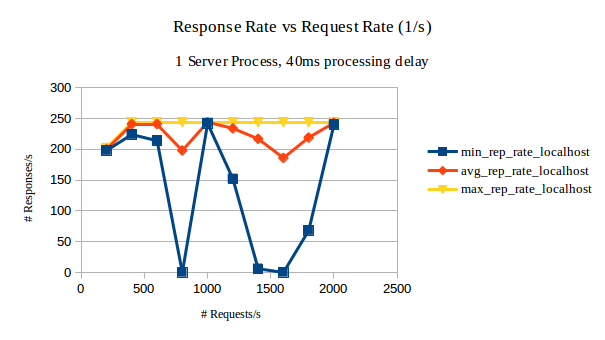
\includegraphics{fig-2-1proc-delay.png}

As expected, when the server was given multiple processes to handle the load, the overall performance increased. When running the web server with 8 worker processes and a 40ms delay in the request processing, the server reached its peak of 2000 responses per second.

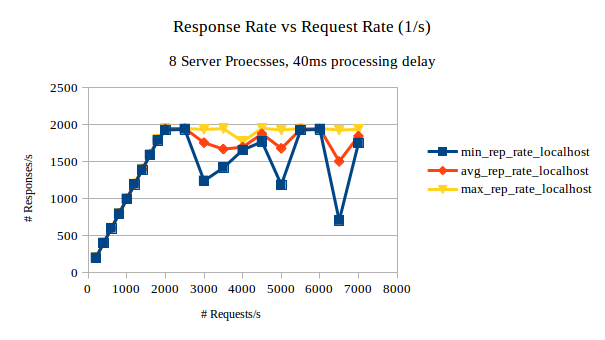
\includegraphics{fig-3-8proc-delay.png}

\subsection{File Serving}
As the requirements for file serving were quite lax, the web server only implements a fixed number of supported files: JPG, JPEG PNG, HTML, CSS, and plaintext (used for all other formats). The final version of the web server is capable of serving these files to the user, providing the necessary details such as content type and content length.

\section{Conclusion}
The major challenge presented in this assignment was the issue of the Erlang benchmarks reporting the same response rates for the single and multi-processed versions of the web server.

It was interesting to learn how Erlang can be leveraged to support multiple connections in parallel, particularly regarding offloading request handling work to new processes.

Implementing the basics of file delivery revealed how much I take for granted when using existing web frameworks.
\end{document}
